\documentclass{easyclass}

\usepackage{todonotes}
\usepackage{mathtools}
\usepackage{cancel}
\usepackage{xfrac}
\usepackage{float}
\usepackage{caption}

\tikzstyle{int}=[draw, fill=blue!20, minimum size=2em]
\tikzstyle{init} = [pin edge={to-,thin,black}]
\tikzstyle{sum} = [draw, fill=blue!20, circle, node distance=1cm]

\begin{document}
\begin{titlepage}
    \university{Politicnico di Milano}
    \courseid{MIDA2}
    \title{Model Identification and Data Analysis \par Part 2}
    \author{Marco Donadoni and Edoardo Morassutto}
    \version{2019 -- 2020}
    \instructor{Instructors:\par Prof. \textsc{Sergio Savaresi}\par
    Ing. \textsc{Stefano Dattilo}}
    \maketitle
\end{titlepage}

\tableofcontents

\chapter{Template}
\section{Table}

\begin{table}[htp]
    \centering
    \begin{tabular}{r|l|p{10cm}}
        Right &  Left  &  Longlonglonglonglonglonglonglong longlonglonglonglonglonglonglonglonglonglonglonglong longlonglonglonglonglong \\
        Right &  Left  &  Longlonglonglonglonglonglong
        longlonglonglonglonglonglonglong
        longlonglonglong
        longlonglonglonglonglonglonglong
    \end{tabular}
    \caption{This is a caption}
    \label{tab:trans-sym}
\end{table}

\section{List}
This is a List:
\begin{itemize}
    \item \textbf{Bullet 1}: Bullet 1 is bullet 1.
    \item \textbf{Bullet 2}: Bullet 2 is bullet 2.
\end{itemize}

\section{Definition}
\begin{definition}\label{def:def1}
\textbf{DEFINITION NAME}: This is a definition.
\end{definition}

% avoid bad break
\vspace{5cm}

\section{Theorem}
\begin{theo}[THEOREM NAME]{theo:theo1}
This is a theorm. Below are equations.
\begin{align}\label{eq:multi-equations}
    \psi(\bvec{a}) &= A\cdot \bvec{a} + \bvec{t}.\\
    R_x &=  \begin{bmatrix}
            0 & \cos(\theta) & -\sin(\theta)\\
            0 & \sin(\theta) & \cos(\theta)\\
            1 & 0 & 0
         \end{bmatrix},
    R_y =  \begin{bmatrix}
            \cos(\theta) & 0 & -\sin(\theta)\\
            \sin(\theta) & 0 & \cos(\theta)\\
            0 & 1 & 0
         \end{bmatrix},
    R_z =  \begin{bmatrix}
            \cos(\theta) & -\sin(\theta) & 0\\
            \sin(\theta) & \cos(\theta) & 0 \\
            0 & 0 & 1
         \end{bmatrix}
\end{align}
\end{theo}

\begin{lem}[LEMMA NAME]{lem:leml}
This is a lemma
\end{lem}

\begin{prf}[LEMMA NAME]{prf:leml}
This is a proof.
\end{prf}

\section{Tikz Pictures}
\begin{figure}[htp]
    \centering
        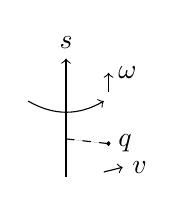
\begin{tikzpicture}[scale=0.6]
            \draw[->] (0,-1)--(0,1.5)node[above] {$s$};
            \draw[->] (-0.8,0.6) to[bend right] (0.8,0.6);
            \draw[->] (0.9, 0.8)--(0.9, 1.2) node[right] {$\omega$};
            \filldraw[dashed] (0,-0.2)--(0.9, -0.3) circle (1pt) node [right] {$q$};
            \draw[->] (0.8, -0.9)--(1.2, -0.8) node[right] {$v$};
        \end{tikzpicture}
    \caption{This is a caption. }
    \label{fig:rotation}
\end{figure}





\curinstructor{Ins Tructor1}

\chapter{Introduction}
\newlecture{Sergio Savaresi}{16/04/2020}

\section{General topics of MIDA course}

\begin{itemize}
    \item Collect digitally data from real systems
    \item Build black-box (gray-box) models from data, with emphasis on
    \begin{itemize}
        \item Dynamic systems
        \item Control/automation-oriented applications
    \end{itemize}
    \item Purpose of modelling (area of machine leasing focusing on ``control'')
    \begin{itemize}
        \item Prediction
        \item Software-sensing
        \item Modelling for control design
    \end{itemize}
\end{itemize}

\subsection{Super summary of MIDA 1}
The focus is on \emph{time series} (output-only systems) and \emph{input/output} (I/O) systems.

Models used in MIDA1:
\begin{itemize}
    \item ARMA models for T.S.
    \item ARMAX models for I/O systems
\end{itemize}

\begin{figure}[H]
    \begin{minipage}[t]{0.4\textwidth}
        \centering
        \begin{tikzpicture}[node distance=2.5cm,auto,>=latex']
            \node [int] (a) {$\frac{C(z)}{A(z)}$};
            \node (b) [left of=a, node distance=2cm] {};
            \node (end) [right of=a, node distance=2cm]{};
            \draw[->] (b) edge node {$e(t)$} (a);
            \draw[->] (a) edge node {$y(t)$} (end);
        \end{tikzpicture}
        \caption*{ARMA model}
    \end{minipage}
    \begin{minipage}[t]{0.4\textwidth}
        \centering
        \begin{tikzpicture}[node distance=2.5cm,auto,>=latex']
            \node [int] (a) {$z^{-k}\frac{B(z)}{A(z)}$};
            \node (b) [left of=a, node distance=2cm] {};
            \node [sum] (c) [right of=a, node distance=2cm] {};
            \node [int] (d) [above of=c, node distance=1.5cm] {$\frac{C(z)}{A(z)}$};
            \node (e) [left of=d, node distance=2cm] {};
            \node (end) [right of=c, node distance=2cm]{};
            \draw[->] (b) edge node {$u(t)$} (a);
            \draw[->] (e) edge node {$e(t)$} (d);
            \draw[->] (a) edge node[pos=0.8] {$+$} (c);
            \draw[->] (d) edge node[pos=0.8] {$+$} (c);
            \draw[->] (c) edge node {$y(t)$} (end);
        \end{tikzpicture}
        \caption*{ARMAX model}
    \end{minipage}
\end{figure}

The model is indicated as $\mathcal{M}(\theta)$ where $\theta$ is the parameter vector, the coefficients of $A(z)$, $B(z)$, $C(z)$.

A \textbf{parametric identification method} has been used: the \emph{performance index is defined}
\begin{definition}
    $J(\theta) = \frac{1}{N} \sum_{t=1}^N \left(y(t) - \hat{y}(t|t-1, \theta)\right)^2$
\end{definition}

Which is the variance of the \emph{prediction error} made by the model. The optimal $\theta$ is $\hat{\theta}_N = \argmin_\theta J(\theta)$

\subsection{MIDA 2}

The focus is on I/O systems (more close to real applications than T.S.).

\begin{description}
    \item[Chapter 1] non-parametric (direct/constructive) black-box identification of I/O systems using state-space models
    \item[Chapter 2] parametric identification fo black-box I/O systems, with a frequency-domain approach
    \item[Chapter 3] Kalman-filter for Sw-sensing using feedback on white-box models
    \item[Chapter 4] black-box methods for SW-sensing without feedback
    \item[Chapter 5] gray-box system identification using Kalman-filter and using \emph{simulation-error methods} (S.E.M,)
    \item[Chapter 6] Minimum-Variance Control (M.V.C.), design of optimal feedback controllers using the theory background of the MIDA course
    \item[Appendix] Recursive (online) implementation of algorithms for system identification
\end{description}

\section{Motivation example for the course: ABS}

\begin{definition}
    \textbf{Slip} of the wheel: $\lambda = \frac{v-\omega r}{v}$
\end{definition}

During a break $0 \le \lambda \le 1$ (from free rolling wheel to locked wheel).
\begin{figure}[H]
    \centering
    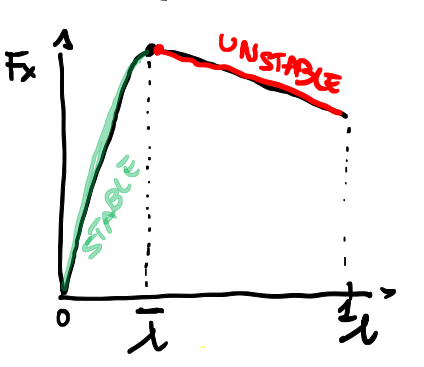
\includegraphics[width=0.5\textwidth]{lectures/2020-04-16/lambda-graph.png}
    \caption*{Relation between $\lambda$ and the breaking force.}
\end{figure}

\begin{figure}[H]
    \centering
    \begin{tikzpicture}[node distance=2.5cm,auto,>=latex']
        \node [int] (abs) {ABS algo};
        \node [sum] (sum) [left of=abs, node distance=2cm] {};
        \node (in) [left of=sum, node distance=2cm] {};
        \node [int] (sys) [right of=abs, node distance=3cm]{System};
        \node [coordinate] (split) [right of=sys, node distance=2cm]{};
        \node (end) [right of=sys, node distance=4cm]{};
        \node [int] (sws) [below of=sys, node distance=1cm]{SW-sensing};

        \draw[->] (in) edge node {$\overline{\lambda}$} (sum);
        \draw[->] (sum) edge node {} (abs);
        \draw[->] (abs) edge node {$u(t)$} (sys);
        \draw[->] (sys) edge node[pos=0.8] {$\lambda$} (end);
        \draw[->] (split) |- node {} (sws);
        \draw[->] (sws) -| node[pos=0.9] {$-$} (sum);
    \end{tikzpicture}
    \caption*{ABS system}
\end{figure}

The problem can be divided into subproblems:
\begin{itemize}
    \item Model of the system
    \item SW-estimation of $\lambda$ ($v$ is not directly measurable, so $\lambda$ cannot be computed)
    \item Design of the ABS control algorithm
\end{itemize}

Why black-box modelling?
The control variable $v$ (the voltage to the actuator) controls a complex systems from the actuator to $\lambda$.
The system can be seen as a chain of components:
\begin{itemize}
    \item Current dynamics and electric motor
    \item Position dynamics of the actuator
    \item Dynamics of the hydraulic circuit of the break system
    \item Tire dynamics
    \item Wheel rotational dynamics
    \item Vehicle full dynamics
\end{itemize}

White box (physical) modelling: write the equations from \emph{first principles}.

Black box modelling: experiment $\rightarrow$ collect data $\rightarrow$ build model.
Using only I/O measured data we can \emph{learn} a mathematical model of the I/O behavior of the system.

\chapter{Black-box non-parametric identification of I/O systems using state-space models}

\begin{figure}[H]
    \centering
    \begin{tikzpicture}[node distance=2.5cm,auto,>=latex']
        \node [int, ellipse] (sys) {system};
        \node (in) [left of=sys, node distance=2cm] {};
        \node (noise) [above of=sys, node distance=1.5cm] {};
        \node (end) [right of=sys, node distance=2cm]{};

        \draw[->] (in) edge node {$u(t)$} (sys);
        \draw[->,dotted] (noise) edge node {$d(t)$ \emph{(not measured disturbance)}} (sys);
        \draw[->] (sys) edge node {$y(t)$} (end);
    \end{tikzpicture}
\end{figure}

\textbf{Measured data}
\begin{align*}
    \left\{u(1), u(2), \ldots, u(N)\right\} &\quad \text{(input)} \\
    \left\{y(1), y(2), \ldots, y(N)\right\} &\quad \text{(output)}
\end{align*}

\begin{remark}[general path of a parametric identification methods]
\end{remark}

\begin{enumerate}
    \item Collect data: $\left\{u(1), u(2), \ldots, u(N)\right\}$, $\left\{y(1), y(2), \ldots, y(N)\right\}$
    \item Select \textbf{a-priori} a class/family of parametric models: $\mathcal{M}(\theta)$
    \item Select \textbf{a-priori} a performance index (it gives an order to the quality of the models)
    \item Optimization step (minimize $J(\theta)$ w.r.t $\theta$): $\hat{\theta}_N = \argmin_\theta J(\theta)$ $\rightarrow$ optimal model $\mathcal{M}(\hat{\theta}_N)$
\end{enumerate}

$J(\theta): \RR^{n_\theta} \rightarrow \RR^+$ (where $n_\theta$ is the order of the model).

$\mathcal{M}(\theta_1)$ is better than $\mathcal{M}(\theta_2)$ if $J(\theta_1) < J(\theta_2)$.

In this chapter we are presenting a totally different system identification approach: \textbf{not parametric}.
\begin{itemize}
    \item No a-priori model-class selection
    \item No performance index definition
    \item No optimization task
\end{itemize}

\section{Representations}

\subsection{Representation \#1: state-space}

\[
\begin{cases}
    x(t+1) = F x(t) + G u(t) & \qquad \text{state equations} \\
    y(t+1) = H x(t) + D u(t) & \qquad \text{output equations}
\end{cases}
\]

Where $F$, $G$, $H$ and $D$ are matricies defined as follows:
\begin{align*}
    F = \begin{bmatrix}
        \\
        n \times n \\
        \text{state matrix} \\ \\
    \end{bmatrix}
    &
    \qquad
    G = \begin{bmatrix}
        \\
        \\
        n \times 1 \\
        \text{input} \\
        \text{matrix} \\ \\
    \end{bmatrix}
    \\ \\
    H = \begin{bmatrix}
        1 \times n \;\;\; \text{output matrix}
    \end{bmatrix}
    &
    \qquad
    D = \begin{bmatrix}
        1 \times 1 \;\;\; \text{i/o matrix}
    \end{bmatrix}
\end{align*}

Assuming 1 input and 1 output, it can be extended for multiple inputs and outputs. Usually $D=0$ for \emph{strictly-proper systems}.

\begin{remark}[S.S representation is not unique]
    $F_1 = TFT^{-1}$, $G_1 = TG$, $H_1 = HT^{-1}$, $D_1 = D$ for any invertible matrix $T$. The system $\{F, G, H, D\}$ is equivalent to $\{F_1, G_1, H_1, D_1\}$.
\end{remark}

\begin{example}
    \[
        \begin{cases}
            x_1(t+1) = \frac{1}{2} x_1(t) + 2u(t) \\
            x_2(t+1) = x_1(t) + 2x_2(t) + u(t) \\
            y(t) = \frac{1}{4}x_1(t) + \frac{1}{2}x_2(t)
        \end{cases}
    \]
    In this case $n=2$, $x(t) = \begin{bmatrix}
        x_1(t) \\
        x_2(t)
    \end{bmatrix}$, one input $u(t)$ and one output $y(t)$.

    \begin{align*}
        F = \begin{bmatrix}
            \frac{1}{2} & 0 \\
            1 & 2
        \end{bmatrix}
        & \qquad
        G = \begin{bmatrix}
            2 \\ 1
        \end{bmatrix}
        \\
        H = \begin{bmatrix}
            \frac{1}{4} & \frac{1}{2}
        \end{bmatrix}
        & \qquad
        D = 0
    \end{align*}
\end{example}

\subsection{Representation \#2: transfer-function}

\[
    W(z) = \frac{B(z)}{A(z)} z^{-k} = \frac{b_0 + b_1z_{-1} + b_2z^{-2} + \ldots + b_pz^{-p}}{a_0 + a_1z^{-1} + a_2z^{-2} + \ldots + a_nz^{-n}} z^{-k}
\]

$W(z)$ is a rational function of the \emph{z} operator: it's a \emph{digital filter}.

It's very easy to move from T.F. representation to a time domain description of the system.

\begin{example}
    \begin{align*}
        & y(t) = \underbrace{\begin{bmatrix}
            \frac{1+\frac{1}{2}z^{-1}}{2+\frac{1}{3}z^{-1}+\frac{1}{4}z^{-2}} z^{-1}
        \end{bmatrix}}_{W(z)} u(t) \\
        & 2y(t) + \frac{1}{3}y(t-1) + \frac{1}{4}y(t-2) = u(t-1) + \frac{1}{2}u(t-2) \\
        & y(t) = \underbrace{-\frac{1}{6}y(t-1) - \frac{1}{8}y(t-2)}_\text{old values of $y(t)$} + \underbrace{\frac{1}{2}u(t-1) + \frac{1}{4}u(t-2)}_\text{old values of input}
    \end{align*}

\end{example}

\begin{remark}[Strictly proper systems]
    Notice that for strictly proper systems the delay $k \ge 1$
\end{remark}
\missingfigure{Graphs about strictly proper systems}

\subsection{Representation \#3: convolution of the input with the Impulse Response (IR)}
The third way to represent a system is through the convolution of the input with the \emph{Impulse Response (IR)}.
\missingfigure{Graphs about convolution}
It can be proven that the input-output relationship from $u(t)$ to $y(t)$ can be written as
\[ y(t) = \omega(0) u(t) + \omega(1) u(t-1) + \omega(2) u(t-2) + \cdots \]
It can be rewritten as follows
\[ y(t) = \sum_{k=0}^{\infty} \omega(k) u(t-k) \]
From this, it is clear that $y(t)$ is the convolution of IR with the input signal.
\missingfigure{Block diagram of system}

\section{Transformation between representations}
\missingfigure{Figure of translation between representations}
\subsection{State Space to Transfer Function}
Consider a strictly proper system with the following state space representation:
\[
\begin{cases}
    x(t+1) = F x(t) + G u(t)\\
    y(t) = H x(t) + \cancelto{0}{D u(t)}\\
\end{cases}
\Rightarrow
\begin{cases}
    x(t+1) = F x(t) + G u(t)\\
    y(t) = H x(t)\\
\end{cases}
\]
From the system we get
\[ z x(t) = F x(t) + G u(t) \Rightarrow x(t) = (zI - F)^{-1} G u(t) \]
\[ \Rightarrow y(t) = H (zI - F)^{-1} G \cdot u(t) \]
Thus, the transfer function is
\[ W(z) = H(zI - F) ^ {-1} G \]

\begin{example}
\begin{align*}
    F = \begin{bmatrix}
        1 & 0\\
        \frac{1}{2} & 2\\
    \end{bmatrix}
    &&
    G = \begin{bmatrix}
        1\\
        1\\
    \end{bmatrix}
    &&
    H = \begin{bmatrix}
        1 & 0\\
    \end{bmatrix}
    &&
    D = 0
\end{align*}
\begin{align*}
W(z) &=
\begin{bmatrix}
    1 & 0\\
\end{bmatrix}
\left( \begin{bmatrix}
    z & 0\\
    0 & z\\
\end{bmatrix}
-
\begin{bmatrix}
    1 & 0 \\
    \frac{1}{2} & 2\\
\end{bmatrix}\right)^{-1}
\begin{bmatrix}
    1\\
    1\\
\end{bmatrix}
= \begin{bmatrix}
    1 & 0\\
\end{bmatrix}
\begin{bmatrix}
    z-1 & 0\\
    -\frac{1}{2} & z-2\\
\end{bmatrix}^{-1}
\begin{bmatrix}
    1\\
    1\\
\end{bmatrix}\\
&= \begin{bmatrix}
    1 & 0\\
\end{bmatrix}
\frac{1}{(z-1)(z-2)}
\begin{bmatrix}
    z-2 & 0\\
    \frac{1}{2} & z-1\\
\end{bmatrix}
\begin{bmatrix}
    1\\
    1\\
\end{bmatrix}
=
\frac{1}{(z-1)(z-2)}
\begin{bmatrix}
    z-2 & 0\\
\end{bmatrix}
\begin{bmatrix}
    1\\
    1\\
\end{bmatrix}\\
&=
\frac{\cancel{z-2}}{(z-1)\cancel{(z-2)}} = \frac{1}{z-1} = \frac{1}{1-z^{-1}} z^{-1}
\end{align*}
Notice that in this case we only have one pole, but the system is of order two; this comes from the fact that part of the system is non observable.

\end{example}

\subsection{Transfer Function to State Space}
This conversion is not very used in practice and it is called the \emph{realization} of a transfer function into a state space model.

Note that the state space representation is not unique, so from a single transfer function we can get infinite different equivalent state space models.

\subsubsection{Control realization}

We assume that the system is strictly proper and that the denominator is monic.
\[ W(z) = \frac{b_0 z^{n-1} + b_1 z^{n-2} + \dots + b_{n-1}}{z^n + a_1 z^{n-1} + a_2 z^{n-2} + \dots + a_n} \]

The formula for the control realization of $W(z)$ is
\begin{align*}
    F = \begin{bmatrix}
        0 & 1 & 0 & \cdots & 0\\
        0& 0 & 1 & \ddots & \vdots \\
        \vdots & \vdots & \ddots & \ddots & 0\\
        0 & 0 & \cdots & 0 & 1\\
        -a_n & -a_{n-1} & \multicolumn{2}{c}{\cdots} & -a_1\\
    \end{bmatrix}
    &&
    G = \begin{bmatrix}
        0\\
        0\\
        0\\
        \vdots\\
        1\\
    \end{bmatrix}
    &&
    H = \begin{bmatrix}
        b_{n-1} & b_{n-2} & \cdots & b_0\\
    \end{bmatrix}
    &&
    D = 0
\end{align*}
\begin{example}
    Consider the transfer function $W(z)$
    \[ W(z) = \frac{2z^2 + \frac{1}{2}z + \frac{1}{4}}{z^3 + \frac{1}{4}z^2 + \frac{1}{3}z + \frac{1}{5}} \]
    The control realization is
    \begin{align*}
        F = \begin{bmatrix}
            0 & 1 & 0\\
            0 & 0 & 1\\
            -\frac{1}{5} & -\frac{1}{3} & -\frac{1 }{4}\\
        \end{bmatrix}
        &&
        G = \begin{bmatrix}
            0\\
            0\\
            1\\
        \end{bmatrix}
        &&
        H = \begin{bmatrix}
            \frac{1}{4} & \frac{1}{2} & 2\\
        \end{bmatrix}
        &&
        D = 0
    \end{align*}
\end{example}

\subsection{Transfer Function to Impulse Response}
To get the IR from a transfer function $W(z)$ is sufficient to make the $\infty$-long division between the numerator and denominator of $W(z)$
\begin{example}
    Consider the transfer function
    \[ W(z) = \frac{1}{z-\frac{1}{2}} = \frac{z^{-1}}{1-\frac{1}{2}z^{-1}}
        = 0 z^{-0} + 1 z^{-1} + \frac{1}{2}z^{-2} + \frac{1}{4}z^{-3} + \cdots \]
    Thus the IR is $\omega(0) = 0$, $\omega(1) = 1$, $\omega(2) = \frac{1}{2}$, $\omega(3) = \frac{1}{4}$, $\dots$

    In this case there is also a quicker way
    \[ y(t) = \frac{z^{-1}}{1-\frac{1}{2}z^{-1}} u(t) = \left( z^{-1} \frac{1}{1-\frac{1}{2}z^{-1}} \right) u(t) \]
    Remembering that for geometric series we have \[ \sum_{k = 0}^{\infty} a^k = \frac{1}{1-a} \text{ if } |a| < 1 \]
    We can rewrite $y(t)$ as follows
    \[ y(t) = \left( z^{-1} \sum_{k=0}^{\infty} \left( \frac{1}{2} z^{-1} \right)^{k} \right) u(t) = \left( 0 + 1 z^{-1} + \frac{1}{2}z^{-2} + \frac{1}{4}z^{-3} + \cdots \right) u(t) \]
\end{example}

\subsection{Impulse Response to Transfer Function}
\begin{definition}
    Given a discrete-time signal $s(t)$ such that $\forall t < 0: s(t) = 0$, its \emph{Z-Transform} is defined as
    \[ \mathcal{Z} \left( s(t) \right) = \sum_{t = 0}^{\infty} s(t) z^{-t} \]
\end{definition}
Given this, it can be proven that
\[ W(z) = \mathcal{Z}\left( \omega(t) \right) = \sum_{t = 0}^{\infty} \omega(t) z^{-t} \]
This means that the transfer function of a system is the $\mathcal{Z}$-transform of a special signal, that is the impulse response of the system.

\begin{remark}
    This formula cannot be used in practice to transform an IR representation to a TF representation.
    This is because we need infinite points of the impulse response, and the impulse response must be noise-free.
    Thus, this transformation is only theoretical.
\end{remark}

\subsection{State Space to Impulse Reponse}
Consider the following state space model, with initial conditions $x(0) = 0$ and $y(0) = 0$
\[
    \begin{cases}
        x(t+1) = F x(t) + G u(t)\\
        y(t) = H x(t)\\
    \end{cases}
\]
We have that
\begin{align*}
    x(1) &= \cancelto{0}{F x(0)} + G u(0) = G u(0)\\
    y(1) &= H x(1) = H G u(0)\\
\end{align*}
\begin{align*}
    x(2) &= F x(1) + G u(1) = F G u(0) + G u(1)\\
    y(2) &= H x(2) = H F G u(0) + H G u(1)\\
\end{align*}
\begin{align*}
    x(3) &= F x(2) + G u(2) = F^2 G u(0) + F G u(1) + G u(2)\\
    y(3) &= H x(3) = H F^2 G u(0) + H F G u(1) + H G u(2)\\
\end{align*}
This can be generalized to
\[ y(t) = 0 u(t) + H G u(t-1) + H F G u(t-2) + H F^2 G u(t-3) + \cdots \]
Thus, the impulse response is
\[
    \omega(t) =
    \begin{cases}
        0 \text{ if } t = 0\\
        H F^{t-1} G \text{ if } t > 0\\
    \end{cases}
\]

\subsection{Summary of transformations}
Notice that the IR representation is very easy to obtain experimentally, since we only need to measure the system response to the impulse signal.
However, given the IR representation, it is difficult to get to the other representations, since the transformation between from IR to TF is only theoretical.
Moving from the IR to the SS representation is the key task of the \emph{Subspace-based State Space System Identification}, also known as \emph{4SID methods}.

\section{Subspace-based State Space System Identification (4SID)}
The original 4SID method starts from the measurement of the system output in a very simple experiment, that is the \emph{impulse experiment}.
\missingfigure{Impulse response}
The fundamental idea is that it is very simple to make this experiment, that is to measure the output of system given an impulse signal as the input.
The real problem is to identify a model $\left\{ \hat{F}, \hat{G}, \hat{H} \right\}$ starting from $\left\{ \omega(0), \omega(1), \omega(2), \cdots \right\}$.

We will see the solution of this problem in two steps:
\begin{enumerate}
    \item IR measurement is assumed to be noise-free.
    This is easier with respect to the original problem, but it is also not realistic.
    \item IR is measured with noise
    \[ \widetilde{\omega}(t) = \omega(t) + \eta(t) \quad t = 0, 1,\dots, N \]
    \begin{itemize}
        \item $\widetilde{\omega}(t)$ is the measured noisy IR
        \item $\omega(t)$ is the ``true'' noise-free IR
        \item $\eta(t)$ is the measurement noise (e.g. WN)
    \end{itemize}
\end{enumerate}
\begin{remark}
    We will see in detail only 4SID when the experiment is an impulse-experiment, which is the first and original version of 4SID.
    However 4SID can be extended to any generic input signal $\left\{ u(1), u(2), \cdots, u(N) \right\}$ that is sufficiently exciting.
\end{remark}
\begin{remark}[Unstable system]
    In case of an unstable system the measurements must be collected in a closed-loop experiment.
    Indeed, if the experiment was open-loop, the experiment would be unfeasible.
    \missingfigure{Unstable system}
    \missingfigure{Closed loop system}
\end{remark}

%\bibliography{bibfile}

\end{document}
